\documentclass[frontgrid]{flacards}
\usepackage{color}
% For funky database symbols
\usepackage{newlfont}
\usepackage{tabularx}
\usepackage{graphicx}

\definecolor{light-gray}{gray}{0.75}

\newcommand{\frontcard}[1]{\textcolor{light-gray}{\colorbox{light-gray}{$#1$}}}
\newcommand{\backcard}[1]{#1} 

\newcommand{\flashcard}[1]{% create new command for cards with blanks
    \card{% call the original \card command with twice the same argument (#1)
        \let\blank\frontcard% but let \blank behave like \frontcard the first time
        #1
    }{%
        \let\blank\backcard% and like \backcard the second time
        #1
    }%
}

\begin{document}

\pagesetup{2}{4} 

\card{
	What is $\sigma$?
}{
	The selection operator (selects rows).
}

\card{
	What is $\pi$?
}{
	The projection operator (selects columns).
}

\card{
	What is $\delta$?
}{
	The distinct operator (makes sure no rows are repeated).
}

\card{
	What is $\times$?
}{
	The product operator (produces all permutations of the rows of two tables).
}

\card{
	What is $\Join$?
}{
	The join operator (natural or otherwise, it joins two tables together based
	on a column).
}

\card{
	What is $\rho$?
}{
	The rename operator (renames column names).
}

\card{
	What are the three layers of DBMS abstraction?
}{
	Physical, logical and view
}

\card{
	Name three DBMS interface languages
}{
	\begin{tabularx}{0.32\textwidth}{l X}
		- & DDL: Data Definition Language\\
		- & DML: Data Manipulation Language\\
		- & DQL: Data Query Language\\
	\end{tabularx}
}

\flashcard{
	To select the age column from the people table without duplicates you would do:\\
	\texttt{SELECT \blank{DISTINCT} \blank{age} FROM \blank{people};}
}

\flashcard{
	To select all the columns of people who are above 50 you would do:\\
	\texttt{SELECT * FROM \blank{people} WHERE \blank{age > 50};}
}

\flashcard{
	To select all the columns of people who are between 20 and 40 you would do:\\
	\texttt{SELECT * FROM \blank{people} WHERE \blank{age BETWEEN 20 AND 40};}
}

% NEED TO ADD MORE SQL FLASHCARDS HERE

\card{
	What are the three main constructs in ER modelling?
}{
	Entity types, attribute types \& relationship types.
}

\card{
	What type of attribute is the following?\\
	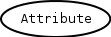
\includegraphics{images/simpleAttribute.png}
}{
	Simple attribute
}

\card{
	What type of attribute is the following?\\
	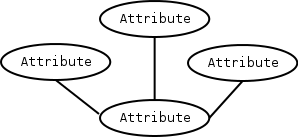
\includegraphics[scale=0.6]{images/compositeAttribute.png}
}{
	Composite attribute
}

\card{
	What type of attribute is the following?\\
	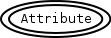
\includegraphics{images/multiAttribute.png}
}{
	Multi-valued attribute
}

\card{
	What type of attribute is the following?\\
	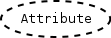
\includegraphics{images/derivedAttribute.png}
}{
	Derived attribute
}

\card{
	What type of entity is the following?\\
	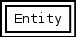
\includegraphics{images/weakEntity.png}
}{
	Weak entity
}

% RELATIONSHIP FLASHCARDS

\end{document} 
